\documentclass{report}
\usepackage{graphicx}

\begin{document}

% Pagina di Copertina
\begin{titlepage}
    \centering
    \vspace*{\fill}
    \Huge \textbf{THESIS TITLE}
    \vspace{2cm} 
    
    \Large Lorenzo Ferrari

    \vspace{2cm} % Spazio aggiuntivo tra il nome e il nome dell'istituto
    
    \Large Università degli studi di Parma
    \par
    Three-year degree course in Computer Science
    
 
\end{titlepage}

%indice
\renewcommand{\contentsname}{Index}
\tableofcontents
    
    
    
    %overview 
    \chapter{overview}
    introduction and some stuff
    % Capitolo buffer overflow
    \chapter{Buffer Overflow vulnerability}
    \section{background} %---------------------fix this text ------------------
    Buffer overflow is a critical vulnerability that emerged around the 1970s and 1980s where it was 
    realized through research which leads the attacker to uncontrolled access to critical points of memory.\newline
    As the 1990s arrived the explosion of the Internet and its client-server infrastructure led large numbers of people to use buffer overflow.\newline
    Furthermore, in this period the first books were published explaining how buffer overflow works.\newline
    In the 2000s people wanted to defend themselves from these types of attacks and invented two types of mitigations:\newline
    \begin{itemize}
        \item[$\bullet$] ASLR (Address Space Layout Randomization)
        \item[$\bullet$] stack canary 
    \end{itemize}
    We will explain this mitigation later.\newline
    Between 2000s and 2010s even with the mitigations attackers managed to avoid them and still exploit buffer overflow vulnerability with technique called:\newline
        \begin{itemize}
        \item[$\bullet$] ROP (Return Oriented Programming)
        \item[$\bullet$] RET2LIBC (Return to Libc)
    \end{itemize}
    Even though vulnerability was born so many years ago it still is one of the biggest an dangerous vulnerablity.
    \clearpage
    %-----------------fix until here--------------------
    \section{How Buffer Overflow works}
    A buffer overflow occurs when the attacker can write more input than expected from the buffer, the overflow input exceeds in the memory in the location right after the buffer we are allocating, this could be very dangerous.\newline
    here's an example:
    \begin{verbatim}
    #include <iostream>
    
    int main() {
    
        char buff[30]; // buffer victim 
        printf(" insert your name: ");
        scanf("%50s",buffS); 
        return 0;
    }
    \end{verbatim}
    In this example we can see a bad usage of a scanf function. In fact, this program has a char buffer with a size of 30, but the scanf function can read up to 50 chars.\newline 
    What happens if we insert more input than expected for the buffer?\newline
    State of the buffer before inserting input:
       
    \begin{figure}[h]
    \centering

    \includegraphics[width=13cm]{Organigrammi.png}
    \caption{Empty stack}
    \label{fig:example_empty_buffer}
    \end{figure}
       \clearpage
    In the example, we can notice that we have our buffer instantiated.\newline
    I wrote the question marks instead of 0x0000000000000000 because this memory at the beginning of the program is instantiated for the program we are executing, but this memory had previously been used in other contexts.\newline
    Now we will try to insert the following paylaod:
    \begin{verbatim}
        AAAAAAAAAAAAAAAAAAAAAAAAAAAAAAPPBBBBBBBBCCCCCCCC
    \end{verbatim}
    i used the "A" to fill the buffer "P" for the remaining buffer before RBP, "B" for overwriting the saved base pointer,
    C for overwriting the return address.
    this will cause a buffer overflow because when we get to the assembly instruction leave and ret it will not find the instruction 0x4343434343434343 and the program will receive a segmentation fault.
    \begin{figure}
        \centering
        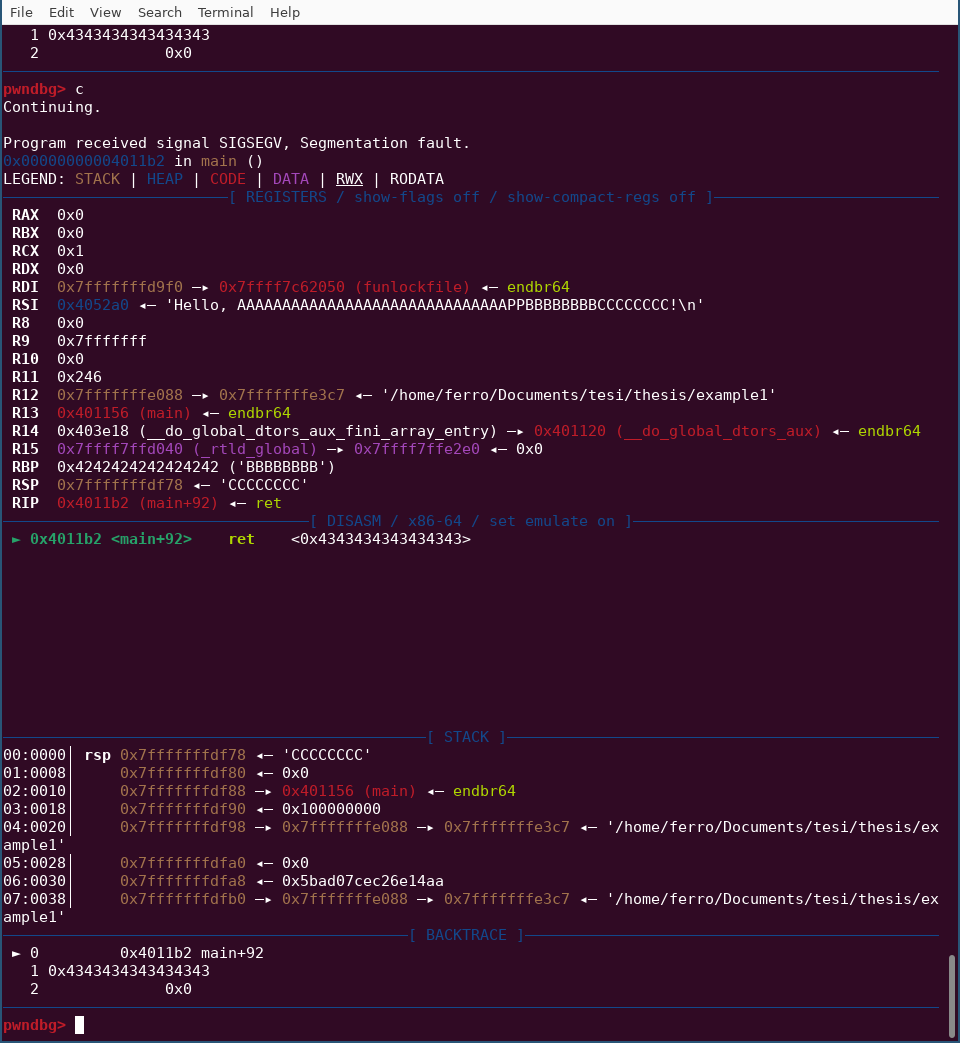
\includegraphics[width=1.3\linewidth]{example1.png}
        \caption{buffer overflow triggered}
        \label{fig:enter-label}
    \end{figure}
    \clearpage
    \section{mitigations against Buffer Overflow}
    mitigazioni buffer overflow
    \clearpage
    \section{Buffer Overflow attack and mitigations bypass}
    to be continued
    \clearpage
    \section{explanation of a challange and exploit analyses}
    to be continued
    
    
    %capitolo heap overflow 
    \chapter{Heap Overflow Vulnerability}
    \section{How it works a Heap Overflow}
    to be continued
    \clearpage
    \section{overview challenge and attack planning}
    to be continued
    \clearpage
    \section{exploit analisys}
    to be continued
    \clearpage
    %capitolo double free
    \chapter{Double Free Vulnerability}
    \section{How it works a Double Free}
    to be continued    
    \clearpage
    \section{overview challenge and attack planning}
    to be continued
    \clearpage
    \section{exploit analisys}
    to be continued
    \clearpage
    % capitolo conclusioni
    \chapter{Conclusion}
    to be continued
    \clearpage
\end{document}
